\documentclass[12pt,a4paper]{article}
\usepackage[utf8]{inputenc}
\usepackage[T1]{fontenc}
\usepackage{amsmath}
\usepackage{amssymb}
\usepackage{lmodern}
\usepackage{upquote}
\usepackage{graphicx}
\usepackage[dvipsnames]{xcolor}
\usepackage{placeins}
\usepackage{float}
\usepackage[left=1.4cm, right=1.4cm, top=2.4cm, bottom=2.20cm]{geometry}
\usepackage{times}
\usepackage{tabularx}
\usepackage{setspace}
\usepackage{multirow}
\usepackage{tikz}
\usetikzlibrary{positioning, arrows.meta, calc, fit, backgrounds}
\usepackage[colorlinks=true, linkcolor=blue, urlcolor=cyan]{hyperref}
\setlength{\parindent}{0pt}
\setlength{\parskip}{0.9em}
\usepackage{fancyhdr}
\usepackage{datetime}
\usepackage{enumitem}

\let\oldheadrule\headrule
\renewcommand{\headrule}{\color{BrickRed}\oldheadrule}
\renewcommand{\headrulewidth}{1.5pt}

\newdateformat{monthyeardate}{%
  \monthname[\THEMONTH], \THEYEAR}

\fancypagestyle{firstpage}{%
  \fancyhf{}
  \fancyfoot[C]{\thepage}
  \renewcommand{\headrulewidth}{0pt}% no header rule on page 1
}

\begin{document}

% ---- Running header for pages 2+ ----
\pagestyle{fancy}
\fancyhf{}
\fancyhead[L]{\small\textit{Juan Zurita --- Research Statement}}
\fancyfoot[C]{\thepage}

% ---- Page 1: no header text, just the title block ----
\thispagestyle{firstpage}

\vspace{-0.2cm}

\begin{center}
{\LARGE {\color{BrickRed}{\textsc{Juan Zurita}}}} \\
\vspace{0.5em}
\textbf{{\Large \textsc{Research Statement}}}
\\
\vspace{0.5cm}
{\small{\textcolor{blue}{juan.zurita@ed.ac.uk} \ $\cdot$ \href{https://juanignaciozurita.github.io/personalwebsite/}{\textcolor{blue}{juanignaciozurita.github.io/personalwebsite}}}}\\
\vspace{-0.0cm}
\begin{tabular}{c @{}}
	\monthyeardate\today
\end{tabular}
\end{center}
\vspace{-1cm}
{\color{BrickRed}\rule{\textwidth}{2pt}}

My research investigates how financial frictions on both sides of the credit market---households and banks---shape the transmission of macroeconomic policy. Combining narrative identification, smooth-transition VARs, high-frequency monetary surprises, and quantitative structural models, I address two central questions: how do balance-sheet constraints alter the potency of monetary and fiscal policy, and who bears the real burden of bank capital regulation? My work spans three interconnected agendas: household debt and policy transmission, banking heterogeneity and credit supply, and fiscal sustainability. Figure~\ref{fig:agenda} maps the connections across these areas.

%==================================================================
\subsection*{Household Debt and Policy Transmission}
\vspace{-0.3cm}

Standard New Keynesian frameworks assign no role to household debt in the transmission of aggregate policy. Central banks---including the RBA, Riksbank, and Norges Bank---have long suspected otherwise. My research provides new empirical evidence for this view and identifies the mechanisms at work.

In \textit{``Does Household Debt Affect the Transmission Mechanism of Monetary Policy?''} (\textbf{Macroeconomic Dynamics}, 2026), I estimate a smooth-transition VAR (STVAR) on data from Australia, Sweden, Norway, and the G7. Two primary results emerge: first, the short-run output response to monetary easing is roughly 0.06 percentage points of GDP \emph{larger} when household debt is elevated, as indebted households are highly sensitive to cash-flow changes. Second, high debt \emph{reduces the persistence} of the stimulus over 4--8 quarters as debt-service obligations reassert themselves.

The fiscal counterpart, \textit{``Does Household Debt Affect the Size of the Fiscal Multiplier?''} (\textbf{Macroeconomic Dynamics}, 2024), reveals a mirror image: government-spending multipliers are larger when household debt is \emph{low}---by 0.70, 0.61, and 0.79 percentage points of GDP on impact in Australia, Norway, and the United States, respectively. Highly indebted households prioritize balance-sheet repair, saving rather than consuming the income generated by fiscal expansions.

Together, these papers establish household balance sheets as a first-order state variable for macro policy: the effectiveness of monetary and fiscal interventions critically depends on the economy's position in the debt cycle.

In \textit{``Household Debt and Low Labour Productivity''} (working paper, 2025), I examine the micro-foundations of this mechanism using Australian administrative microdata. Middle-aged mortgagors facing debt-service ratios above 20 percent respond to rising obligations by increasing labour supply. In an incomplete-markets model, this labour-supply response amplifies short-run output responsiveness on the extensive margin but increases structural fragility to subsequent macroeconomic shocks. The household balance sheet shapes the supply side of the economy, not just the demand side.

%==================================================================
\subsection*{Banking, Credit Supply, and Regulation}
\vspace{-0.3cm}

If the potency of macro policy depends on the debt cycle, then who controls the credit pipeline matters enormously. Three papers analyze the supply side---the banking sector.

\paragraph{Banking heterogeneity and growth.} In \textit{``Banking Heterogeneity, Credit Supply and Economic Growth''} (\textbf{International Review of Economics and Finance}, 2026), I compile a novel dataset matching over 5,000 U.S.\ bank balance sheets to loan-level mortgage and commercial data. I show that standard macro models ignoring lender heterogeneity severely understate credit transmission: accounting for bank equity-size distribution amplifies the estimated impact of mortgage lending on local GDP growth by up to \emph{sixty times}, and business lending by up to \emph{eighteen times}. The architecture of the financial system, not just its aggregate size, determines how credit affects the real economy.

\paragraph{Who bears the burden of bank capital regulation? (Job Market Paper)} My job market paper asks who actually pays when regulators tighten capital requirements. Using narratively identified capital-requirement shocks and a quarterly panel of approximately 4,800 U.S.\ banks (1994--2019), I show that the burden is organised by two variables that appear on every bank's balance sheet---and in no statute. \emph{Within} banks, commercial lending contracts about a third more than real-estate lending, reflecting differential risk weights. \emph{Across} banks, institutions with thin voluntary capital buffers cut lending most: the buffer gradient is approximately 1.3 times, extending well beyond the two percent of bank-quarters at the regulatory frontier.

The sharpest finding concerns the instrument regulators actually control. Statutory size tiers---the basis of current tailoring---explain under two percent of the cross-sectional variance in regulatory slack, and eighty-six percent of the banks in the thinnest-buffer tercile face the \emph{lowest} statutory requirement. The statute sorts banks by size; the mechanism sorts them by buffer. The two sorts are nearly orthogonal.

A heterogeneous macro-banking model with precautionary buffers reproduces the buffer gradient as an untargeted moment (1.32 in the model against 1.32 in the data). Risk weights and size tiers redistribute the burden of a tightening but barely change its aggregate magnitude---a gross transition cost excluding the stability benefits of capital. The macroeconomic cost is governed by the \emph{level} of requirements, not their design.

\paragraph{The bank profit channel of monetary policy.} In joint work with Jiening Le (submitted, 2026), we show how monetary policy tightening impacts bank profitability across the size distribution. High-frequency monetary surprises linked to Call Report data reveal a stark non-linear effect: a one-standard-deviation increase in expense-channel exposure compresses net interest income by 9 percent for small banks and 11 percent for large banks, but peaks at \emph{19 percent} for mid-sized banks. This reflects a liability-substitution channel: mid-sized banks lack both the cheap deposit retention of small banks and the flexible wholesale funding access of money-center banks. The profitability squeeze persists for several quarters, implying that tightening cycles constrict credit supply disproportionately through mid-sized lenders.

%==================================================================
\subsection*{Fiscal Sustainability}
\vspace{-0.3cm}

Fiscal consolidation does not happen in a vacuum---the tax instruments governments choose interact with the credit cycle I study elsewhere, affecting household disposable income and, through it, debt-service capacity. As Principal Investigator on a Royal Society of Edinburgh grant, I examine whether structural productivity gains can substitute for fiscal discipline in the United Kingdom (\textit{``Labour Productivity Growth and the Fiscal Sustainability Programme in the United Kingdom,''} working paper, 2025). Within a DSGE framework, I show that maintaining real government spending per worker without expanding the debt-to-GDP ratio necessitates higher taxation regardless of productivity growth. The tax-mix analysis reveals that capital taxes repair the fiscal deficit but severely impair long-run growth, consumption taxes create volatility, and labour taxes represent the least distortive consolidation instrument---practical guidance for any advanced economy navigating the tension between spending commitments and debt sustainability.

%==================================================================
\subsection*{Future Agenda}
\vspace{-0.3cm}

My future research bridges household credit demand with institutional bank credit supply---closing the gap between the two pillars of my existing work:

\begin{itemize}[nosep, leftmargin=1.5em]\itemsep0.3em
\item \textit{Earnings risk and cyclical credit dynamics} (with Emiliano Carlevaro): We study how earnings risk varies over the business cycle in a volatile economy and interacts with household portfolio choices and bank balance-sheet constraints. Using Argentine administrative employer--employee data, we are assembling a panel of earnings histories to estimate the cyclicality of idiosyncratic risk. If earnings risk is countercyclical, households demand more precautionary credit precisely when the banking sector is least willing to supply it---a mechanism absent from current heterogeneous-agent models.

\item \textit{Macroprudential policy in a two-sided debt economy}: I am developing a general-equilibrium framework where regulatory shocks to bank capital interact dynamically with the household debt cycle. Tighter capital rules reduce credit supply; high household debt dampens the demand-side absorption of fiscal attempts to offset the contraction. The two amplification mechanisms should reinforce each other, with implications for the design of joint monetary-macroprudential rules. This project directly unifies the demand-side findings of my \textit{Macroeconomic Dynamics} papers with the supply-side mechanisms of the JMP.
\end{itemize}

%==================================================================
\vspace{0.1cm}
\begin{figure}[H]
\centering
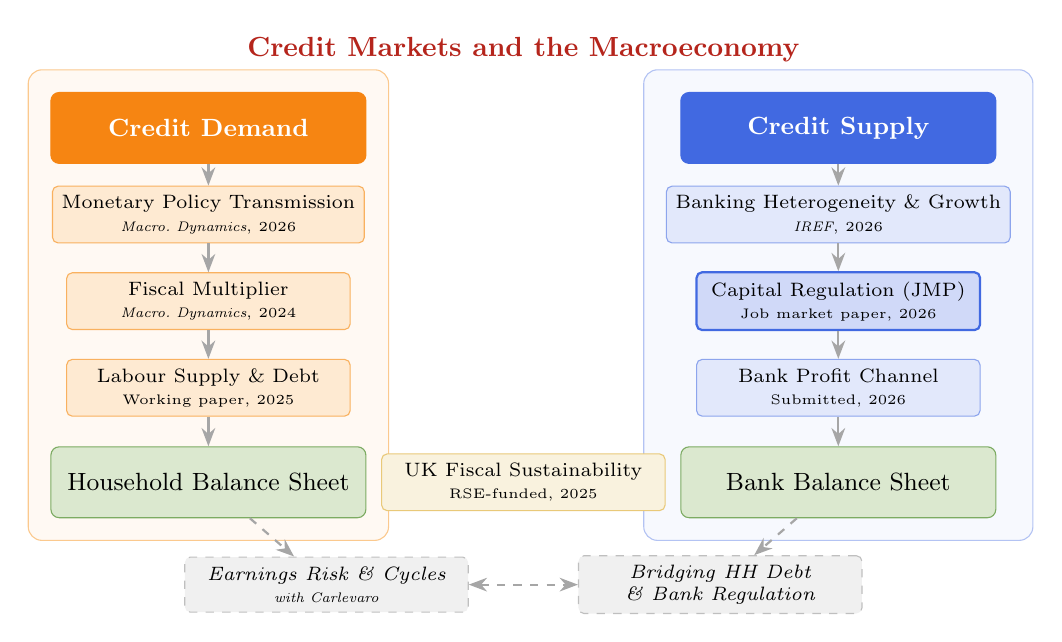
\begin{tikzpicture}[
    >=Stealth,
    node distance=1.2cm and 1.8cm,
    box/.style={rectangle, draw, rounded corners=3pt, minimum width=3.2cm, minimum height=0.9cm, align=center, font=\small},
    bigbox/.style={rectangle, draw, rounded corners=3pt, minimum width=3.6cm, minimum height=1cm, align=center, font=\small\bfseries},
    heading/.style={rectangle, fill=#1, draw=#1, rounded corners=3pt, minimum width=4cm, minimum height=0.9cm, align=center, font=\small\bfseries, text=white},
    paper/.style={rectangle, fill=#1!15, draw=#1!60, rounded corners=2pt, minimum width=3.6cm, minimum height=0.7cm, align=center, font=\scriptsize},
    future/.style={rectangle, fill=Gray!12, draw=Gray!50, rounded corners=2pt, dashed, minimum width=3.6cm, minimum height=0.7cm, align=center, font=\scriptsize\itshape},
    arr/.style={->, thick, color=Gray!70},
]

% ---- Credit Market label ----
\node[font=\normalsize\bfseries, color=BrickRed] (title) at (0, 4.8) {Credit Markets and the Macroeconomy};

% ---- Two pillars ----
\node[heading=BurntOrange] (demand) at (-4, 3.8) {Credit Demand};
\node[heading=RoyalBlue] (supply) at (4, 3.8) {Credit Supply};

% ---- Demand-side papers ----
\node[paper=BurntOrange] (mp) at (-4, 2.7) {Monetary Policy Transmission \\ \tiny\textit{Macro.\ Dynamics}, 2026};
\node[paper=BurntOrange] (fp) at (-4, 1.6) {Fiscal Multiplier \\ \tiny\textit{Macro.\ Dynamics}, 2024};
\node[paper=BurntOrange] (ls) at (-4, 0.5) {Labour Supply \& Debt \\ \tiny Working paper, 2025};

% ---- Supply-side papers ----
\node[paper=RoyalBlue] (bh) at (4, 2.7) {Banking Heterogeneity \& Growth \\ \tiny\textit{IREF}, 2026};
\node[paper=RoyalBlue, fill=RoyalBlue!25, draw=RoyalBlue, line width=0.8pt] (jmp) at (4, 1.6) {Capital Regulation (JMP) \\ \tiny Job market paper, 2026};
\node[paper=RoyalBlue] (bpc) at (4, 0.5) {Bank Profit Channel \\ \tiny Submitted, 2026};

% ---- Connecting theme ----
\node[box, fill=OliveGreen!15, draw=OliveGreen!60, minimum width=4cm] (hh) at (-4, -0.7) {Household Balance Sheet};
\node[box, fill=OliveGreen!15, draw=OliveGreen!60, minimum width=4cm] (bank) at (4, -0.7) {Bank Balance Sheet};

% ---- Fiscal (separate strand) ----
\node[paper=Goldenrod] (fiscal) at (0, -0.7) {UK Fiscal Sustainability \\ \tiny RSE-funded, 2025};

% ---- Future ----
\node[future] (f1) at (-2.5, -2.0) {Earnings Risk \& Cycles \\ \tiny with Carlevaro};
\node[future] (f2) at (2.5, -2.0) {Bridging HH Debt \\ \& Bank Regulation};

% ---- Arrows: demand side ----
\draw[arr] (demand) -- (mp);
\draw[arr] (mp) -- (fp);
\draw[arr] (fp) -- (ls);
\draw[arr] (ls) -- (hh);

% ---- Arrows: supply side ----
\draw[arr] (supply) -- (bh);
\draw[arr] (bh) -- (jmp);
\draw[arr] (jmp) -- (bpc);
\draw[arr] (bpc) -- (bank);

% ---- Arrows: future bridging ----
\draw[arr, dashed] (hh) -- (f1);
\draw[arr, dashed] (bank) -- (f2);
\draw[arr, dashed, <->] (f1) -- (f2);

% ---- Bounding boxes ----
\begin{scope}[on background layer]
  \node[fit=(demand)(mp)(fp)(ls)(hh), inner sep=8pt, draw=BurntOrange!40, fill=BurntOrange!4, rounded corners=5pt] {};
  \node[fit=(supply)(bh)(jmp)(bpc)(bank), inner sep=8pt, draw=RoyalBlue!40, fill=RoyalBlue!4, rounded corners=5pt] {};
\end{scope}

\end{tikzpicture}
\caption{Research agenda: Credit markets and the macroeconomy. Solid arrows trace the progression of completed work; dashed arrows indicate planned projects that bridge the demand and supply sides.}
\label{fig:agenda}
\end{figure}

%==================================================================

\vspace{0.5em}
\rule{5cm}{1pt} \\
Juan Zurita\\
Lecturer in Economics / Early Career Researcher\\
School of Economics, University of Edinburgh\\
30 Buccleuch Place, Newington, Edinburgh EH8 9JT, United Kingdom\\
\textcolor{blue}{juan.zurita@ed.ac.uk} \ $\cdot$ \ \href{https://juanignaciozurita.github.io/personalwebsite/}{\textcolor{blue}{juanignaciozurita.github.io/personalwebsite}}

\end{document}
